
\documentclass[openany]{book}
\usepackage{graphicx} % images
\usepackage{listings} % nice code layout
\usepackage[usenames]{color} % color
\definecolor{listinggray}{gray}{0.9}
\definecolor{graphgray}{gray}{0.7}
\definecolor{ans}{rgb}{1,0,0}
\definecolor{blue}{rgb}{0,0,1}
% \Verilog{title}{label}{file}
\newcommand{\Verilog}[3]{
  \lstset{language=Verilog}
  \lstset{backgroundcolor=\color{listinggray},rulecolor=\color{blue}}
  \lstset{linewidth=\textwidth}
  \lstset{commentstyle=\textit, stringstyle=\upshape,showspaces=false}
  \lstset{frame=tb, tabsize=2}
  \lstinputlisting[caption={#1},label={#2}]{#3}
}
\renewcommand{\chaptername}{Lab}


\title{ELC 3338 Project Book}
\author{Keith Evan Schubert}


\begin{document}

\maketitle
\tableofcontents


\chapter{Introduction}

In the Labs for this course we will be building a 32-bit computer, so we can understand how it works and how we can make a synthesizable machine in a hardware description language (HDL) like Verilog.  In this lab we will be building the counter that sequences all our computer's instructions.

A computer has to execute one instruction after another.  We will be building a system to count sequentially from some starting number.  Since this counter will be used to keep our program running in order, it is called the program counter.  Our system needs to hold its value, count, and be able to change the starting value.  We will break this into three components: a register (to hold the data), an incrementer (to count), and a mux (to select the count or a new starting value).  For today we will just build the register, simulate it, and show how to write up the lab.

\section{Program Counter}

The register is called the program counter, since it holds the actual count.  It is the heart of our system so it is where we will start.  We are going to make a module that explains how to build a register in Verilog.  Consider the code in Listing~\ref{code:register}.  It is made up of three sections: a header (which has the include command), a port list or interface (which specifies the signals coming in or going out of our module), and a body or implementation (which describes how to build it).

\Verilog{Verilog code to make a register.}{code:register}{../code/register.v}

The first part is the header.  We will use this same header each time.  It tells the Verilog compiler to get all the data from a file called definitions.vh.  The extension vh is a Verilog header.  We use this to specify common pieces of data we will use across our design, so that all the components we build will be consistent.  By putting them in one file, we make it easier to maintain, and prevent mistakes that can happen easily by having multiple copies of these basic pieces of data.  For our first component the piece of data we will be using is WORD, which is the size of data our computer will use (how many bits).  We will be using 32-bits, but note that if we build things based around WORD, rather than the number 32, we can just change the value of WORD in the file and get a computer with a different size (say 64) with a couple key strokes.

The second part is the port list or interface.  In this area we specify what signals are coming in (input), going out (output), or could go either direction (inout).  For outputs only, we could also have the output driven by a register (reg) or not (wire).  The other two types (input and inout) are only wires.  If you don't specify anything for any of the port types, you will get a wire - it is the default.  In our case we have four signals: three inputs, and one output that is a register.  The first two inputs are single wires.  One is the clock, which specifies the timing, and the other is reset, which clears the contents (makes the zero).  The final input is the value we want to store in memory, and I have called it D, following the convention of digital logic.  D has multiple bits that are numbered from WORD-1 down to 0.  Thus the leftmost bit is 31 in this case, and the rightmost bit is 0\footnote{If you want to be technical this is called little endian, since the little end (the least significant or unit bit) is going into the first memory location (bit 0).  If you reversed the order by putting the 0 first and the WORD-1 last it would be big endian, since the big end (most significant bit) would go in the lowest addressed bit.}.  If you changed WORD to be 64, this would automatically become 63 down to 0, which would resize the input.  Pretty cool\footnote{I grew up in the 80's so I reserve the right to say cool, rad, tubular, or any other 80's-ism.  :) }!  The output Q (also the digital logic conventional name) is a register (it will hold its value) and should also be of size WORD and follow the same order as the input D.

The final section is the body or implementation.  It is composed of a single thread of code, that will keep running (hence always).  It will run one time every time there is a positive edge (0 to 1 transition) for either the clock or reset.  Reset has higher priority, so if reset is asserted the register is cleared (Q is set to zero), otherwise the value of D is stored it Q.  That is it.  A nice, simple module.

\section{Testbench}

We now want to test this.  To test it, we need to tell the simulator to build a copy (instantiate) the module, and then we will need to supply the inputs and look at the outputs.  Consider the testbench in Listing~\ref{code:register_test}.

\Verilog{Verilog code to test a register.}{code:register_test}{../code/register_test.v}

Like our register it starts with our standard header, but this time there are no ports!  A testbench is providing all the signals to simulate the inputs to the unit under test (UUT) and thus does not need them.  This is how Verilog finds a top level simulation module - there are no ports.  In the body (implementation) we have a bunch of things.  First all the signals to our UUT must be declared.  Outputs always must go to wires (the outputs are driving them, and only wires can be driven).  Often inputs become registers since you will want to specify a value and have it continue till you give it a new value, though some can be wires if you had another unit that was supplying the values from its outputs.  In our case, the clock signal will be driven by a module names oscillator, which will give us a nice square wave with period CYCLE, which is another constant defined in our definitions.vh file.  The code thus makes an oscillator and a register, then runs the initial thread (it runs once at the start then never again)  The initial thread sets the value of the input then waits a CYCLE.  The last couple delays are not full cycles.  I did this for two reasons:
\begin{enumerate}
\item To show you how to make Verilog do calculations for you.
\item To remind you that the input won't necessarily be nice and perfectly timed to your register.  Unsynchronized signals happen, and is a frequent cause of problems, hence the need to test.
\end{enumerate}
This is by no means an exhaustive testbench, but run it and look at the output.  Does it do what you expect?  What else might you want to test?  Add this to your testbench and run it again to see if the register works.



\begin{figure}
\caption{Timing diagram.}\label{fig:registertiming}
\begin{center}
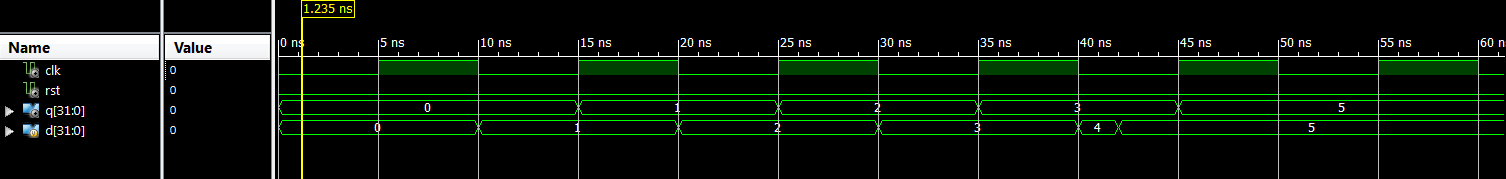
\includegraphics[width=4.75in]{../images/registertiming.png}
\end{center}
\end{figure}

\section{Using \LaTeX\ for Your Write-up}

Alls that is left is to write it up.  I am going to have you use \LaTeX\ to do your labs. Note how I include files, programs, and images.  It is worth noting that \LaTeX\ will automatically make the table of contents and bibliography for you also.  To top it off you only need a text editor as the files are just ASCII files.  To generate the document you run the command pdflatex and pass it the main file, and it will generate a pdf.

Why use \LaTeX\ ?  There are lots, but here are a few that matter in this course
\begin{enumerate}
\item It typesets programs from the actual source, no need to copy the program and have spell checkers and grammar editors mess things up.
\item It quickly and correctly handles equations (important given our math use).
\item It automatically handles table of contents and bibliographies.
\item It is free, and generates high quality documents (book quality) - it is open source since before open source.
\item It is used in publication of research documents.
\item It is the only large program believed to be error free in its source code, and have no missing features (development is complete!)
\end{enumerate}


\subsection{Background}

\TeX\ refers to both a language for typesetting and the program (compiler actually) that does the typesetting.  \LaTeX\ is a macro package which sits on top of \TeX\ and provides additional functionality, and has become synonymous with the language variant (dialect) of \TeX\ which it created.  Since \LaTeX\ is hugely popular and really useful, \TeX\ and \LaTeX\ have become synonymous to most people, and I will treat it so from now on.  A note on pronunciation: \TeX\ is in Greek letters - tau epsilon chi and hence is pronounced `tek' not tex (similar for \LaTeX\, which is pronounced `lay-tek' not latex).

\TeX\ is not a WYSIWYG (what you see is what you get) typesetting program like many editors you are familiar with, as it was designed to be a tagged language like the more recent html (yes, \TeX is older).  The idea is not to spend time thinking about how it should look, but rather to classify what it is and let the automated standards set the text by what the text is\footnote{For instance, note the chapter, section, and subsection commands in the tex files.  \LaTeX\ assigns a number, records it, the title, and page so it can automatically put it in the table of contents for you.}.  To provide flexibility and extension (and it was designed by one of the greatest computer scientists, Donald Knuth) it was set up as a programming language with a compiler.  You will thus interact with several different programs, an ASCII text editor (to write the files), a \TeX\ application to compile them, a pdf or dvi viewer to look at the output, and potential helper apps like dvi2ps, dvi2pdf, and their viewers.  Since \LaTeX\ is a programming language, we have a comment character \% that I had to escape by putting a \textbackslash before it to make it print.  Whitespace past the first space (word separation) is ignored, except for a blank line, which means start a new paragraph.  More than one blank line is ignored.  To get more space, you issue a command, such as \verb1\vspace{.25in}1, which puts a quarter inch of vertical space.  \LaTeX\ also knows pt (points), px (pixels), pc (pica), mm (millimeters), cm (centimeters), em (width of an `m'), and many more.  By default the space is not placed if it does not separate some object (i.e. at the top of a page), but you can force it by using \verb1\vspace*{.25in}1.  Starred commands are just versions of the main command.

There are many more commands than I can describe in this brief intro, including commands to let you define new commands and environments.  We will not need too many fancy commands, we only need to describe the commands to include figures, code, and equations.  If you want to learn more, then I have links to free manuals online at r2labs.org.

\subsection{Compile Process}

One thing that will help you a lot in working with \LaTeX\ is how the compile process works.  \TeX\ is a two pass compiler, but it does only one pass each time it runs.  Allow me a brief introduction to compilers, which is a great course if you can take it.

When you are compiling a file you have control statements (branches, loops, conditional execution statements like if or switch/case) that require you to know how many program lines ahead or behind something is in the assembled code, which you will not know at the start.   While you are often just putting in a flag or label to be handled by the assembler later, you in truth don't even know if they actually put the destination of the transfer of control, and thus have an error.  One easy way of handling this is to run through the process twice, collecting labels and such the first time and then doing the compile the second time through, which is what a two pass compiler does.  \TeX\ collects all the labels, notes all the chapter, section, and other structures, identifies all the bibliography references, and so on and puts them in a special auxiliary file for the next pass.  It will also create a DVI file, which has most things right, but will lack table of contents, references, bibliography, and such.  The second time through it already has the information before the file runs so it reads that first and uses it to create a fully correct output.

A logical question at this point is why not just have it run twice on its own?  Well, in the 1980's computers were small and slow, so each run of \TeX (we didn't even have \LaTeX\ at first) took an appreciable amount of time.  If you know the compile process, there are times you only have to run things once, like small spelling changes not in a title, chapter, etc.  Allowing people to do only one pass at a time was a big advantage (some \TeX\ compiles I had to do could take 10 minutes even in the 1990's).  Bibliographies are handled by an external program called BibTeX, which reads the .aux file to find the references (thus you need to run \LaTeX\ first), then pulls the data from the .bib files you specify in the calling command in your .tex file and creates a .bbl file.  The .bbl file contains all the info formatted how the bibliography should look.  \LaTeX\ reads this in the first pass and copies it over to the .aux file and resolves the links to the text references.  The next run of \LaTeX reads all this in and places both the bibliography and the cross references.  This means that to get a bibliography in you must run \LaTeX\, BibTeX, \LaTeX\, then \LaTeX\ once more.  You only need to do this if you add new reference, which in the labs will be once, provided you don't delete those intermediary files.

\section{Your Assignment}

You are to:
\begin{enumerate}
\item Finish the testbench in Listing~\ref{code:register_test}.
\item Run a simulation and generate a timing diagram like I did.
\item  Write up a lab report in \LaTeX\ following the lab format in \verb1LabN.tex1 and generate a pdf file.
\item Upload the pdf and all the Verilog files to the course LMS.
\end{enumerate} 
%The instructions are stored in memory, and are accessed by using the address where they are stored.  You can think of memory like a giant hotel for our data.  Each piece of data is an integer, and gets stored in a room (memory location), which we can find by its room number (memory address).  To get a piece of data, like an instruction, stored in memory we need to take its address, go to that location, and grab the value.  A bunch of memory locations, accessed by an address is called an array. 
%\input{fetch}
%\input{branching}
%\chapter{ALU and ALU Control}

\section{ALU}

First we will build the ALU itself.  The ALU has three inputs (two data inputs to act on, and a control input to determine the action perfomed) and two outputs (one data, and a logical flag). In Figure~\ref{fig:alubits}
\begin{figure}
\caption{ALU control bit meaning.}\label{fig:alubits}
\begin{center}
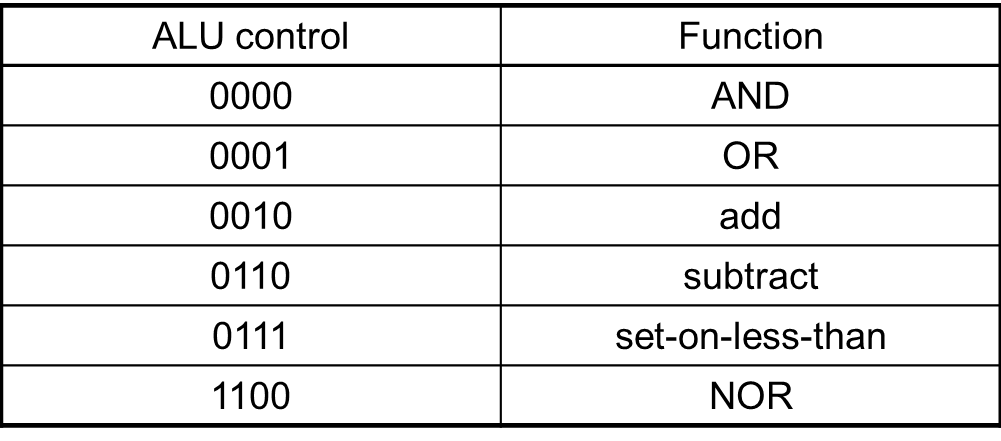
\includegraphics[width=0.6\textwidth]{../images/alubits.png}
\end{center}
\end{figure}
you can see the meaning of the control bits used to determine what the ALU will calculate.  One way to build the ALU is to have it calculate each function and select the one you want.  This is fast and simple but wasteful, thus you would need to determine if speed is a good enough reason to do this.  In our case it is the approach we will take due to the simplicity.  Generating all and selecting indicates a mux, and since there are many options it is a large mux, so a case statement is called for.  The ALU control bits have been given names in the definitions.vh file, so be sure to use them as the individual cases.  Also don't forget to make a default case, which is needed to actually wire this up.  Pick something fast for the default, thus usually a logic statement.

One last thing to note is the generation of the zero flag.  There are several ways to handle this, here are two (you can pick).  
\begin{enumerate}
\item In Verilog (like C), the statement $(a==b)$ is an operation with a boolean output.  You can thus say $x=(a==b);$ to assign $x$ to be the boolean value.  The statement $x=(a==b);$ is realizable as a digital comparator with $a$ and $b$ as inputs and $x$ as the single bit output.
\item Verilog gives you reducing logic by putting the gate before an array of bits, indicating all the bits are to be connected by that logic gate to produce a single output.  This is a particularly elegant gate that is useful in many places including here.  Think how you can determine something is zero by reducing with a gate, then possibly negating.
\end{enumerate}

\section{ALU Control}

Now we need to build the controller to use the ALUOp field and the function field to generate the ALU control bits used above.  Consider the table in Figure~\ref{fig:alucontrolbits}.  
\begin{figure}
\caption{ALU control bit generation.}\label{fig:alucontrolbits}
\begin{center}
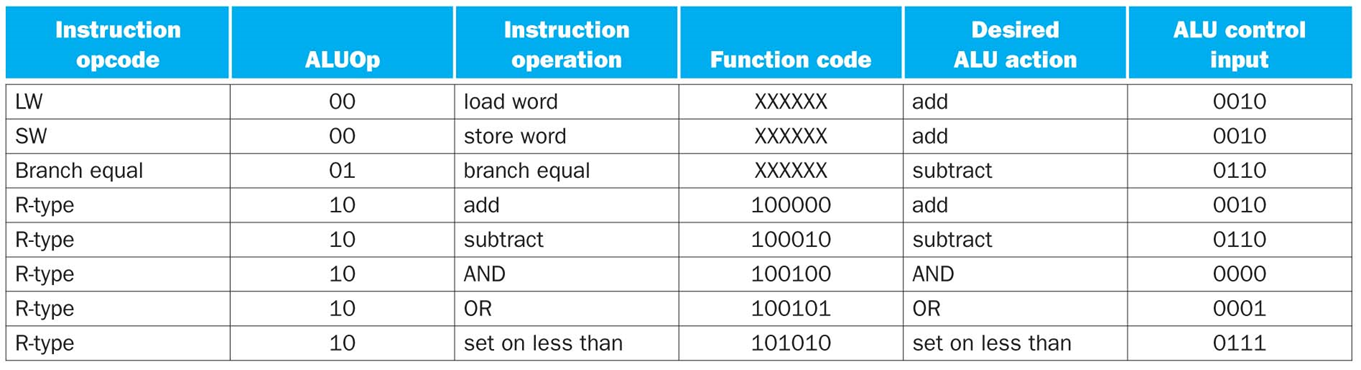
\includegraphics[width=\textwidth]{../images/ALUcontrolbits.png}
\end{center}
\end{figure}
The first two columns are the initial sorting on ALUOp.  The second two columns explain the secondary sorting based on the function field used for R-Type commands.  The final two columns explains what the output of the function should be.  Selecting between many connected values indicates a mux and thus a case statement.  A two layered sorting indicates a nested mux/nested case statement is needed.  Be careful when you code as the nesting is only needed for the R-Type commands.  In both the case statements include a default to handle undefined signals (use fast commands for undefined signals).  Use the signal names defined in the definitions.vh file to improve readability - you shouldn't need any numbers.  This should be a simple module with two inputs (ALUOp and function) and one output (control bits).

\section{Your Assignment}

You are to:
\begin{enumerate}
\item Finish the ALU and ALU control modules.
\item Test both modules with a testbench, run a simulation and generate a timing diagram.
\item  Write up a lab report in \LaTeX\ following the lab format in \verb1LabN.tex1 and generate a pdf file.
\item Upload the pdf and all the Verilog files to the course LMS.
\end{enumerate} 
%\input{multicycle_alu}
%\chapter{Starting to Decode}

In our last lab, you finished the first stage of our pipeline, Fetch, by adding a buffer.  Now we are going to move on to the first two components of the decode stage.

\section{Sign Extender}
Consider the code in Listing~\ref{code:se}.  It really has only one new line, which shows two uses of curly braces: concatenation and replication.  Concatenation is done by \verb1{a,b}1, which would concatenate the bits of a with the bits of b to form a longer sequence.  Replication is done by \verb1n{a}1, which copies a n times.  If you look at our code it takes a number that is half a word long, and makes it a full word by copying the most significant bit.  The replication is made generic by using the constant WORD, and calculating the bit locations.  Unfortunately, the bit location (index) and number of times to copy it (n) have yet to be entered.

\Verilog{Verilog code to build a sign extender.}{code:se}{../code/sign_extender.v}


\section{Control Unit}
The control unit is the brains of our operation.  It will have to take the first six bits of every instruction (the opcode), and set the control bits.

First lets discuss what signals we are setting.  Almost all the boolean signals are described in Figure~\ref{fig:signals}.  The tricky one in the table is PCSrc, which can't be calculated yet, since we need to know whether the condition of the branch was met.  All we know at the moment is that it is a branch, so that is the signal the control will send. Later after the condition has been checked in the execute stage, we can combine the branch signal with the result of the condition to generate PCSrc.  ALUop is not described, though the value of both its bits is, since it is not a boolean signal.  ALUop is a signal that tells the alu control unit, which we will build in the execute stage, what to do or to check the function field.

\begin{figure}
\caption{Control signal meanings and values.}\label{fig:signals}
\begin{center}
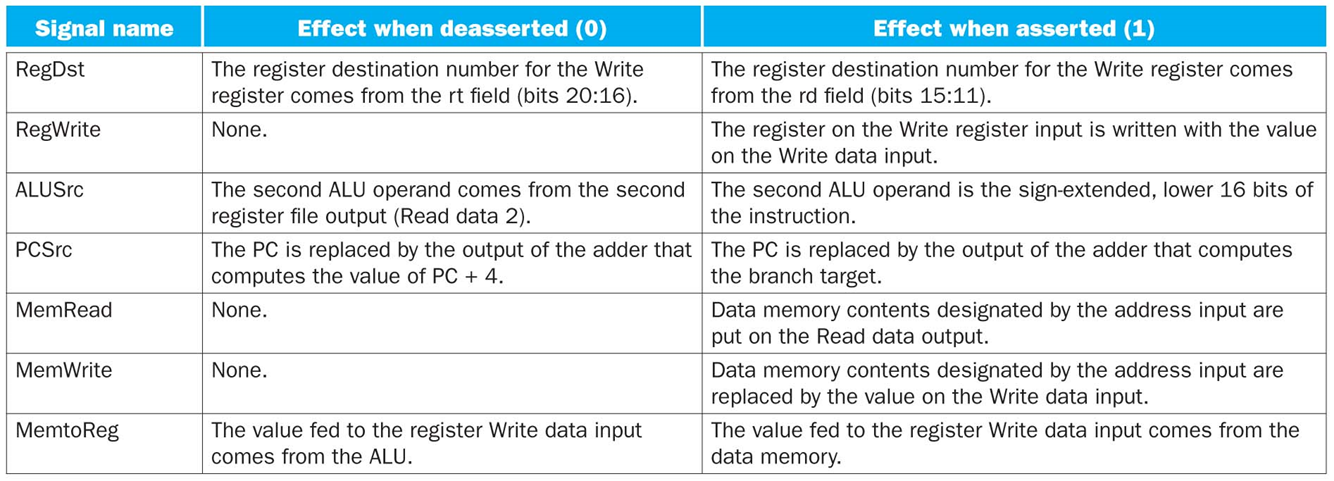
\includegraphics[width=\textwidth]{../images/signal_meaning.png}\\
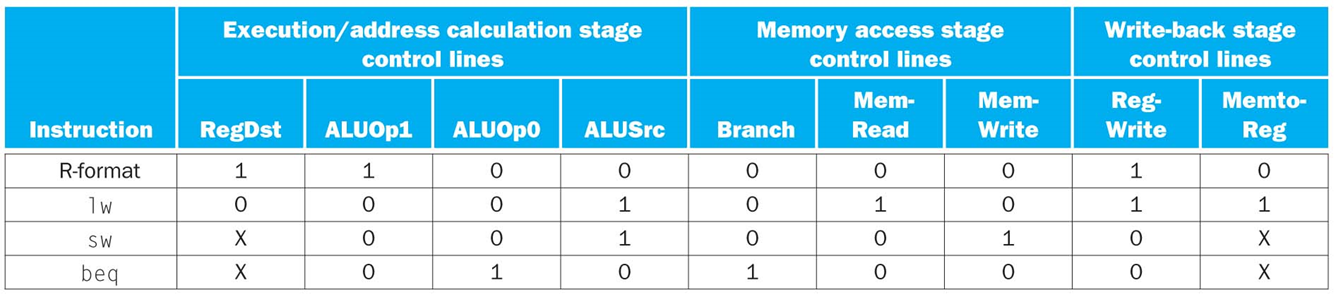
\includegraphics[width=\textwidth]{../images/control_lines.png}
\end{center}
\end{figure}

Consider the code in Listing~\ref{code:control}.  We introduce the switch statement, since it is the fastest way to check an integer indexed group of things, both in hardware and software.  The other well known alternative is a group of nested if-then-else statements.  In hardware\footnote{This is similar for software, where if you code it well you can get log base 2 evaluations on average.} this makes a series of nested 2-input muxes, which means there will be log base 2 levels of muxes to go through.  In complexity lingo, this is $O(\log(n))$ in time (how long it takes), and $O(1)$ in space (how big each mux is).  A case statement is similar to a switch-case statement in C.  In hardware\footnote{In software, this makes a branch table which takes no conditions and only a single branch to resolve!} this makes a single large mux, which thus has only one level of evaluation.  In complexity lingo this is $O(1)$ in time, and $O(n)$ in space.  We care about time, so we will go with the case statement.  Our case statement is missing the signal values, which you can fill in from Figure~\ref{fig:signals}.  Note I have defined the ALUop values as constants to improve readability, so you should use them (see definitions.vh for the names).

\Verilog{Verilog code for the control unit.}{code:control}{../code/control.v}

\section{Your Assignment}

You are to:
\begin{enumerate}
\item Finish the sign extender and control unit.
\item Write a testbench for the sign extender and control unit, run them and generate the timing diagram.
\item  Write up a lab report in \LaTeX\ following the lab format in \verb1LabN.tex1 and generate a pdf file.
\item Upload the pdf and all the Verilog files to the course LMS.
\end{enumerate} 

%midterm
%\input{pipelining}
%\input{performance2}
%\input{forwarding}
%\input{performance3}
%\input{cache}
%\input{performance4}

%\appendix
%\chapter{Overview}

\section{Syllabus Statement}
The building of a computer is an essential aspect in really understanding the material, and as such we will be
building a MIPS computer in an HDL.  Key parts of the project will be discussed and worked on in class but you
must work on aspects as homework to finish.  You will need to test your components by building testbenches and
generating timing diagrams.  You will work in groups of 2-3. When your group is finished you will write a report
documenting what you accomplished.  All project files must be zipped into a single
file and uploaded to the class Blackboard by the end of day on the day marked on the schedule.  If you submit your project
on time, you may re-submit a fixed project for a re-grade.  Stay on top of your project!

\section{Details of Project}

Your MIPS computer, will be a non-pipelined, 32-bit MIPS datapath as discussed in class.  It is to be programmed in VHDL.  Instruction and data cache will be simplified for practicality to a separate instruction and data memory.  It must be able to handle the following commands (identical to the list handed out in class with signal values):
\begin{enumerate}
\item lw
\item sw
\item beq
\item add
\item subtract
\item and
\item or
\item set on less than
\end{enumerate}
The design is to be done at the behavioral level/RTL.  Each of the components of the MIPS Datapath (pc, adders, instruction memory, control, muxes, register file, sign extender, alu, alu control, \textbf{and} gate, data memory, and oscillator) must be clearly defined and the code readable.  You must also create entities for the five stages of the data path, and one for your final complete datapath.  Reset can be grounded unless you use it to initialize memory, in which case you must clearly document this in the design and the report.

Your completed MIPS computer will be tested by initializing the three memory elements to run programs and verifying their outputs.  You should provide an easy way to initialize memory, either by array instantiation in the files or loading external files, both of which were done in class.  It is highly advised that you test your MIPS computer on several programs, as you don't know what will be used to test your code.

Per the syllabus, you are to write a report documenting the results.  One report per group.  List the complete names of everyone in the group.  The report should be in some standard program (Word or {\LaTeX} is preferred).  Make sure the report and all source files are included in the final zip that is uploaded to the course Blackboard site by the end of day on November~10.  There is no page requirement, though shorter is better provided all the required elements are present.    The required elements are:
\begin{enumerate}
\item Give a introduction explaining what a MIPS computer is, aimed a the level of a student in ELC 3338.  Try to keep this to half a page to a page.
\item Explain your design method.  You should include things like the design paradigm (top-down or bottom-up, etc), how the components were selected and grouped, why were you supposed to do this at behavioral level/RTL, how you instantiated the components, and your parameterization/header file scheme and why you did it this way.
\item Explain clearly how to initial memory and why you chose this, anything else you feel would be helpful to grade your design.
\item The way you tested your components, and some screen shots explaining the results.  You can limit this to the ones you had to do outside class.  Explain why you chose the method you did, and the test vectors.  What were the results?  Any lessons learned?
\item Explain the program and data setup for your test program for the entire pipeline and include run data that verifies it worked.  Explain the important points in the run that verified success.
\item State conclusions.  What you learned.  What you would do different.  What you liked or didn't like about this.  I reward those who tell me they didn't like things so don't fear telling me what you feel.  It is very important for your career to be able to state disagreement in a professional manner, as engineers must be able to state problems.
\end{enumerate}


\section{MIPS DataPath}
The MIPS you are building, should look 

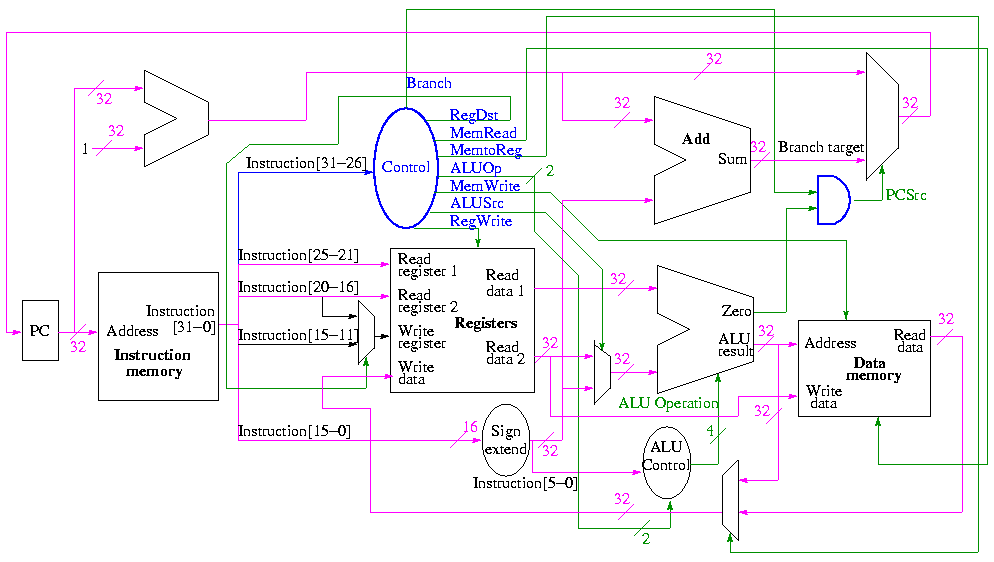
\includegraphics[width=\textwidth]{images/pipeline.png}


\section{MIPS Commands and Format}
\noindent
\begin{tabular}{p{1.25in}|p{.35in}|p{.35in}|p{.35in}|p{.35in}|p{.35in}|p{.35in}|}
  \cline{2-7}
  R-Format            & op & rs   & rt   & rd   & shamt & funct \\ \cline{2-7}
  Bits                & 6  & 5    & 5    & 5    & 5     & 6     \\ \cline{2-7}
  add \$r1,\$r2,\$r3  & 0  & \$r2 & \$r3 & \$r1 & 0     & 32    \\ \cline{2-7}
  addu \$r1,\$r2,\$r3 & 0  & \$r2 & \$r3 & \$r1 & 0     & 33    \\ \cline{2-7}
  sub \$r1,\$r2,\$r3  & 0  & \$r2 & \$r3 & \$r1 & 0     & 34    \\ \cline{2-7}
  subu \$r1,\$r2,\$r3 & 0  & \$r2 & \$r3 & \$r1 & 0     & 35    \\ \cline{2-7}
\end{tabular}

\vspace{.1in}\noindent
\begin{tabular}{p{1.25in}|p{.35in}|p{.35in}|p{.35in}|p{1.38in}|}
  \cline{2-5}
  I-Format             & op & rs   & rt   & address \\ \cline{2-5}
  Bits                 & 6  & 5    & 5    & 16      \\ \cline{2-5}
  lw \$r1,off(\$r2)    & 35 & \$r2 & \$r1 & off     \\ \cline{2-5}
  sw \$r1,off(\$r2)    & 43 & \$r2 & \$r1 & off     \\ \cline{2-5}
  beq \$r1,\$r2, label & 4  & \$r1 & \$r2 & label   \\ \cline{2-5}
\end{tabular}

\noindent
\begin{tabular}{llccc}
Mnemonic & Meaning                                  & Type & Opcode & Funct \\\hline
add	     & Add	                                    & R	   & 0x00   & 0x20 \\
addi     & Add Immediate	                        & I    & 0x08   & NA \\
addiu    & Add Unsigned Immediate	                & I    & 0x09   & NA \\
addu     & Add Unsigned	                            & R    & 0x00   & 0x21 \\
and      & Bitwise AND	                            & R    & 0x00   & 0x24 \\
andi     & Bitwise AND Immediate	                & I    & 0x0C   & NA \\
beq      & Branch if Equal	                        & I    & 0x04   & NA \\
bne      & Branch if Not Equal	                    & I    & 0x05   & NA \\
div      & Divide	                                & R    & 0x00   & 0x1A \\
divu     & Unsigned Divide	                        & R    & 0x00   & 0x1B \\
j        & Jump to Address	                        & J    & 0x02   & NA \\
jal      & Jump and Link     	                    & J    & 0x03   & NA \\
jr       & Jump to Address in Register	            & R    & 0x00   & 0x08 \\
lbu      & Load Byte Unsigned	                    & I    & 0x24   & NA \\
lhu      & Load Halfword Unsigned	                & I    & 0x25   & NA \\
lui      & Load Upper Immediate	                    & I    & 0x0F   & NA \\
lw       & Load Word	                            & I    & 0x23   & NA \\
mfhi     & Move from HI Register	                & R    & 0x00   & 0x10 \\
mflo     & Move from LO Register	                & R    & 0x00   & 0x12 \\
mfc0     & Move from Coprocessor 0 	                & R    & 0x10   & NA \\
mult     & Multiply	                                & R    & 0x00   & 0x18 \\
multu    & Unsigned Multiply     	                & R    & 0x00   & 0x19 \\
nor      & Bitwise NOR (NOT-OR)	                    & R    & 0x00   & 0x27 \\
xor      & Bitwise XOR (Exclusive-OR)	            & R    & 0x00   & 0x26 \\
or       & Bitwise OR	                            & R    & 0x00   & 0x25 \\
ori      & Bitwise OR Immediate	                    & I    & 0x0D   & NA \\
sb       & Store Byte	                            & I    & 0x28   & NA \\
sh       & Store Halfword	                        & I    & 0x29   & NA \\
slt      & Set to 1 if Less Than	                & R    & 0x00   & 0x2A \\
slti     & Set to 1 if Less Than Immediate	        & I    & 0x0A   & NA \\
sltiu    & Set to 1 if Less Than Unsigned Immediate	& I    & 0x0B   & NA \\
sltu     & Set to 1 if Less Than Unsigned	        & R    & 0x00   & 0x2B \\
sll      & Logical Shift Left	                    & R    & 0x00   & 0x00 \\
srl      & Logical Shift Right (0-extended)	        & R    & 0x00   & 0x02 \\
sra      & Arithmetic Shift Right (sign-extended)	& R    & 0x00   & 0x03 \\
sub      & Subtract	                                & R    & 0x00   & 0x22 \\
subu     & Unsigned Subtract	                    & R    & 0x00   & 0x23 \\
sw       & Store Word	                            & I    & 0x2B   & NA \\
\end{tabular}

\vspace{.1in}\noindent
\begin{tabular}{lcp{.2in}lc}\hline
Function          & ALU Control  && Function          & ALU Control  \\\hline
And               & 0000         && Subtract          & 0110         \\
Or                & 0001         && Set on Less Than  & 0111         \\
Add               & 0010         && Nor               & 1100         \\\hline
\end{tabular}

\vspace{.1in}\noindent
\begin{tabular}{|l|ccc|ccc|cc|}\hline
&\multicolumn{3}{|c|}{Ex Stage} &\multicolumn{3}{|c|}{Mem Stage} & \multicolumn{2}{|c|}{W/B Stage} \\\cline{2-9}
            & Reg & ALU & ALU &        & Mem  & Mem   & Reg   & Mem    \\
Instruction & Dst & Op  & Src & Branch & Read & Write & Write & to Reg \\\hline
lw          & 0   & 00  & 1   & 0      & 1    & 0     & 1     & 1      \\
sw          & x   & 00  & 1   & 0      & 0    & 1     & 0     & x      \\\hline
beq         & x   & 01  & 0   & 1      & 0    & 0     & 0     & x      \\
R-Type      & 1   & 10  & 0   & 0      & 0    & 0     & 1     & 0      \\\hline
\end{tabular}

%\chapter{Components From Class}
\Verilog{MUX}{c-mux}{verilog/Keith/mux.v}
\Verilog{Oscillator}{c-osc}{verilog/Keith/oscillator.v}
\Verilog{Register}{c-reg}{verilog/Keith/register.v}
\Verilog{Data Memory}{c-dmem}{verilog/Keith/data_mem.v}
\Verilog{Instruction Fetch Stage}{c-if}{verilog/Keith/iFetch.v}
\Verilog{Instruction Fetch Stage Testbench}{c-ift}{verilog/Keith/iFetch_test.v}

\end{document} 